\subsection{Simplified and original Ikeda method}
\label{se:si_ikeda_model}
Comparing the results from the SI-method from corresponding results with the original Ikeda's method can be a way to see whether the observed deviations are result from extrapolation or inherent in the original method. In Ikeda's method, more detailed information about the ship hull geometry is needed so that $B_W$ can be calculated with a strip method and $B_E$ can be calculated using sectional Lewis coefficients. It was possible to collect the required hull inputs for 15 ships in the database. These ships were used in 50 of the reference roll decay tests: all but one of the tests exceed the limits. Ikeda's method has a much better agreement for these exceeding model tests according to Fig.\ref{fig:si_ikeda_model} and the calculated $R^2$ in Table \ref{tab:si_ikeda_validation}.

\begin{figure}[H]

    \centering
    \includegraphics[width=0.4\textwidth]{figures/si_ikeda_model.eps}
    \caption{Comparison of SI, Ikeda and model tests}
    \label{fig:si_ikeda_model}

\end{figure}

\input{equations/si_ikeda_validation}

